\newcommand{\U}[1]{\ensuremath{\,\textrm{#1}}}
\newcommand{\tref}{\ensuremath{\textrm{ref}}}
\newcommand{\vthref}{\ensuremath{v_\textrm{thref}}}
\newcommand{\gkw}{\ensuremath{\texttt{GKW}}}
\newcommand{\gkdb}{\ensuremath{\texttt{GKDB}}}

\documentclass[a4paper]{report}
\usepackage{fullpage}
\usepackage{amsmath}
\usepackage{amssymb}
\usepackage{bm}
\usepackage{graphicx}
\usepackage{tabularx}
\usepackage{hyperref}

\hypersetup{bookmarks, plainpages=false, colorlinks=true, pdfborder={0 0 0 0}, linkcolor=blue, citecolor=blue, urlcolor=blue, pdftitle={GKDB documentation}}

\begin{document}

\title{Documentation of the GKW to GKDB data conversion}

\author{Y. Camenen on behalf of the GKDB working group}

\date{Last update: February 9, 2018}

\maketitle

\chapter{Preamble}
This document describes how to transform inputs and outputs from a GKW flux-tube simulation to match the format used in the GyroKinetic DataBase (GKDB). \\ 
The reader is assumed to have some knowledge of GKW and to have read the documentation of the GKDB.

\tableofcontents

\chapter{Conventions and normalisations}

\section{Coordinate systems}

In GKW, the toroidal direction is defined to have the cylindrical coordinate system $(R,Z,\varphi)$ right-handed whereas in the GKDB it is defined to have $(R,\varphi,Z)$ right-handed, see Fig.\ref{fig:coord1}. In practice, it means that: 
\begin{equation}
\varphi^\gkw=-\varphi^\gkdb
\end{equation}
\begin{figure}[h]
	\begin{center}
		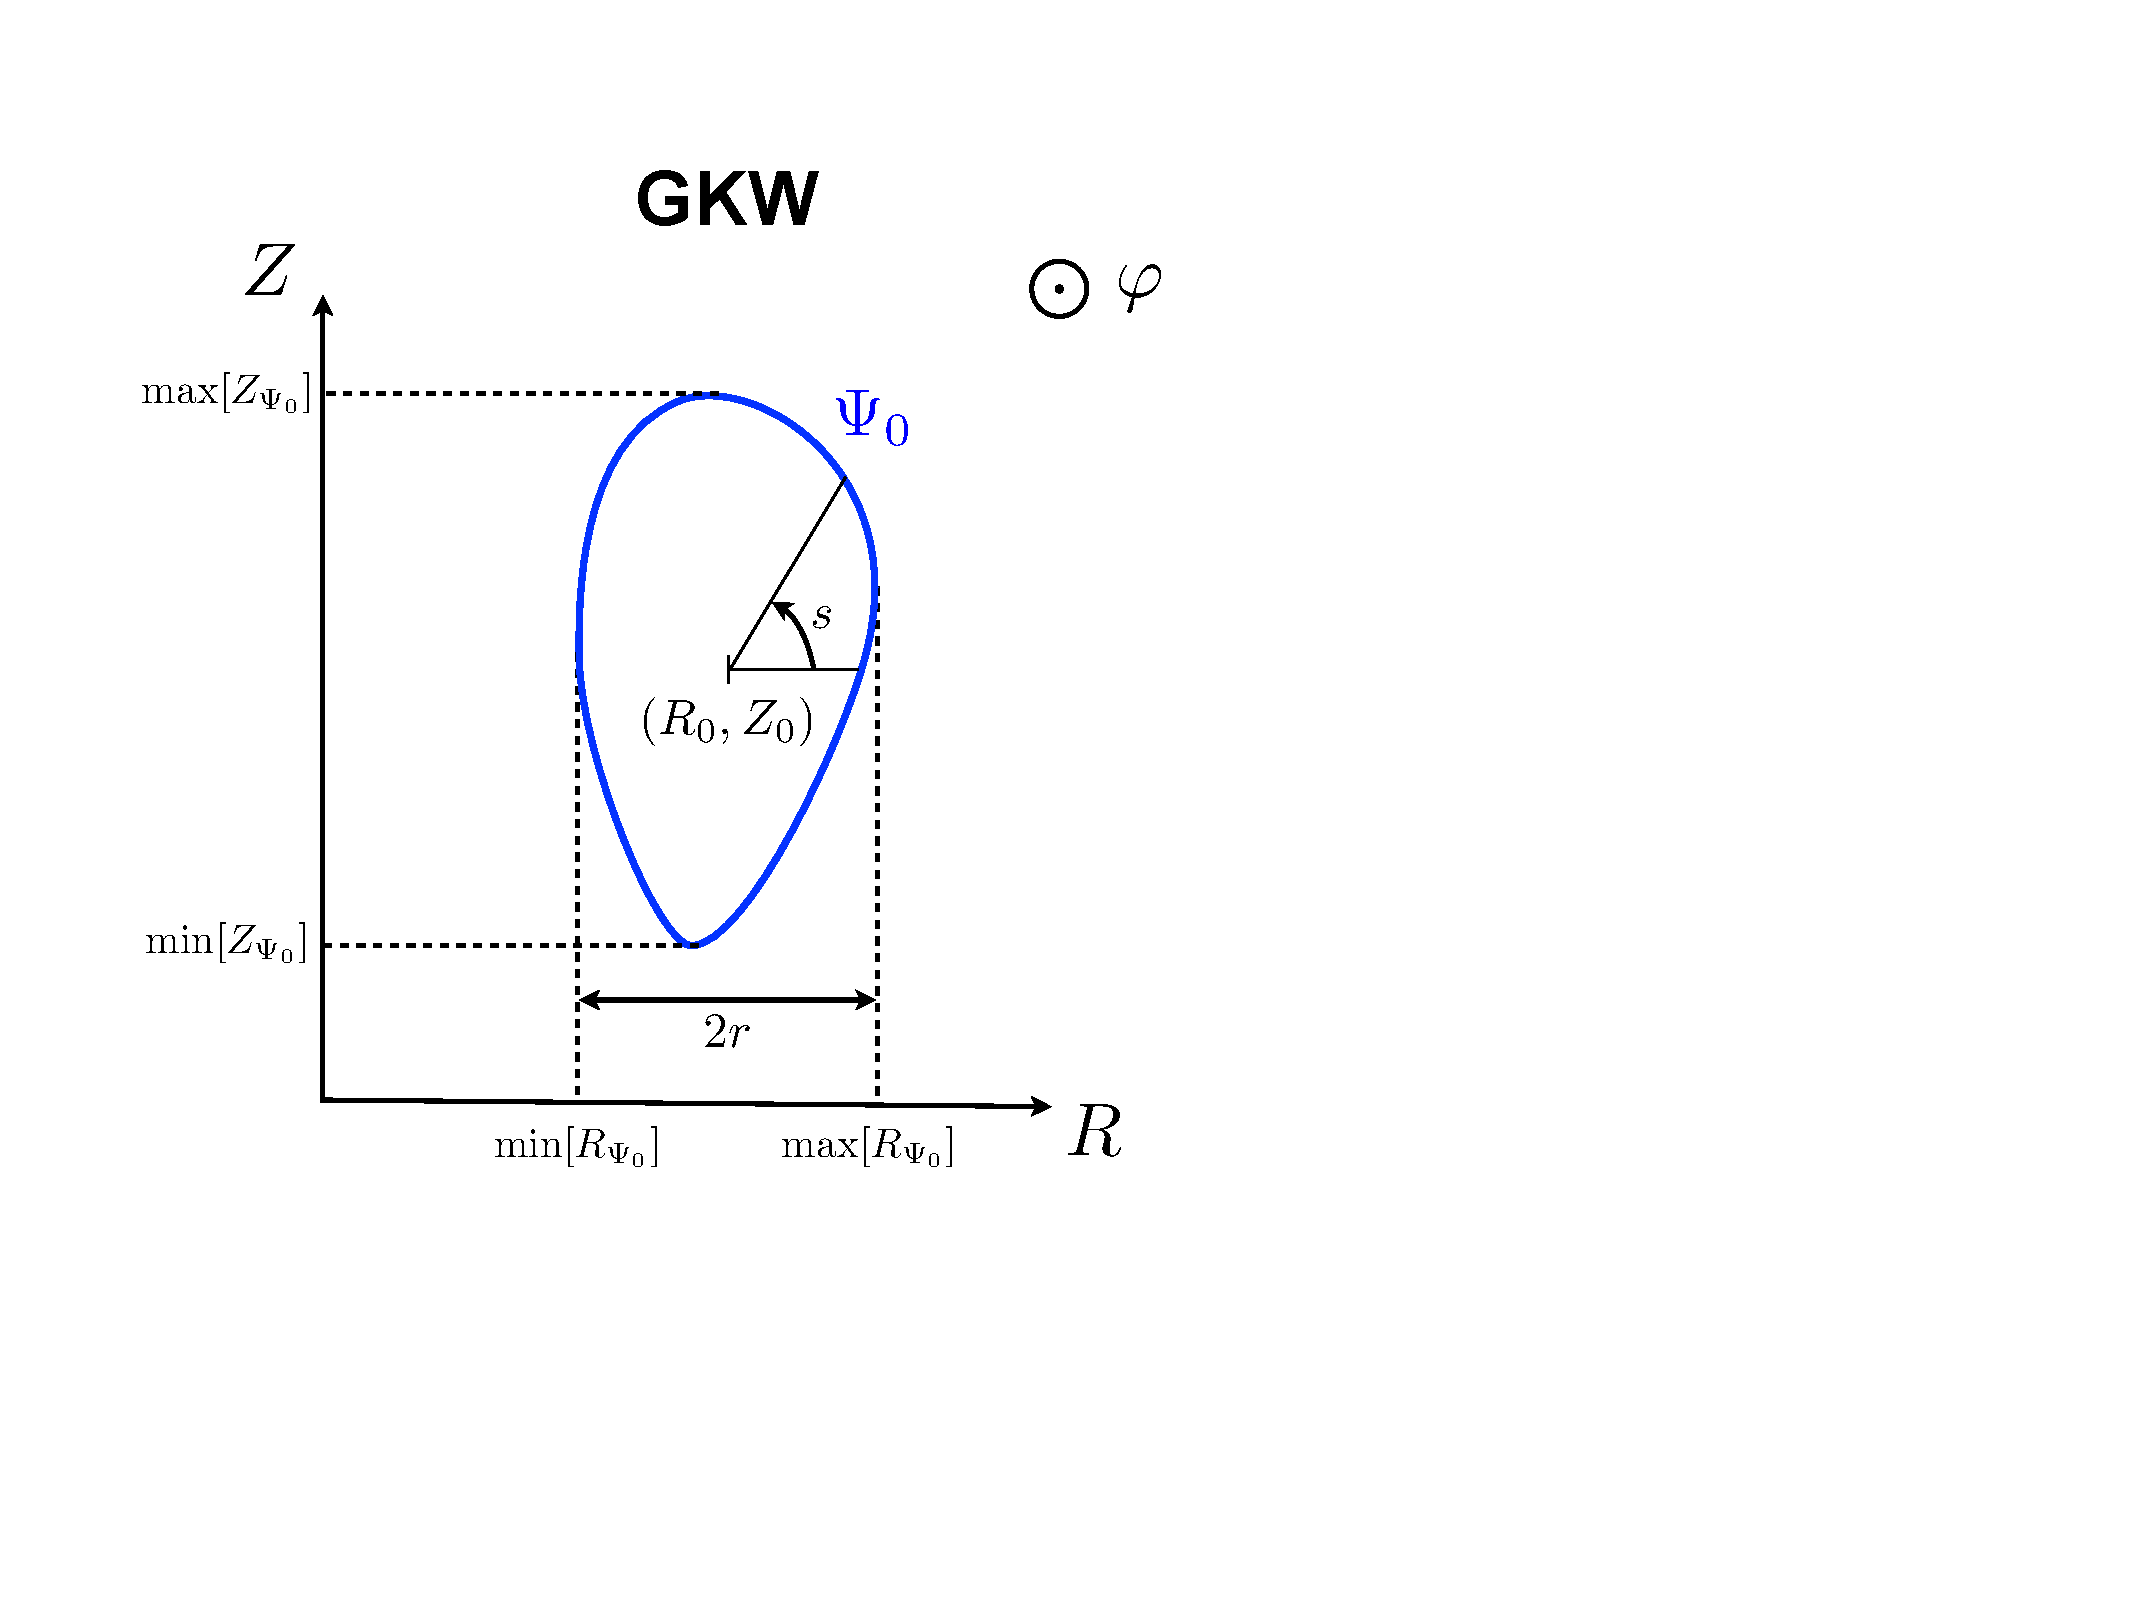
\includegraphics[width=7cm]{GKW_coord.pdf}
		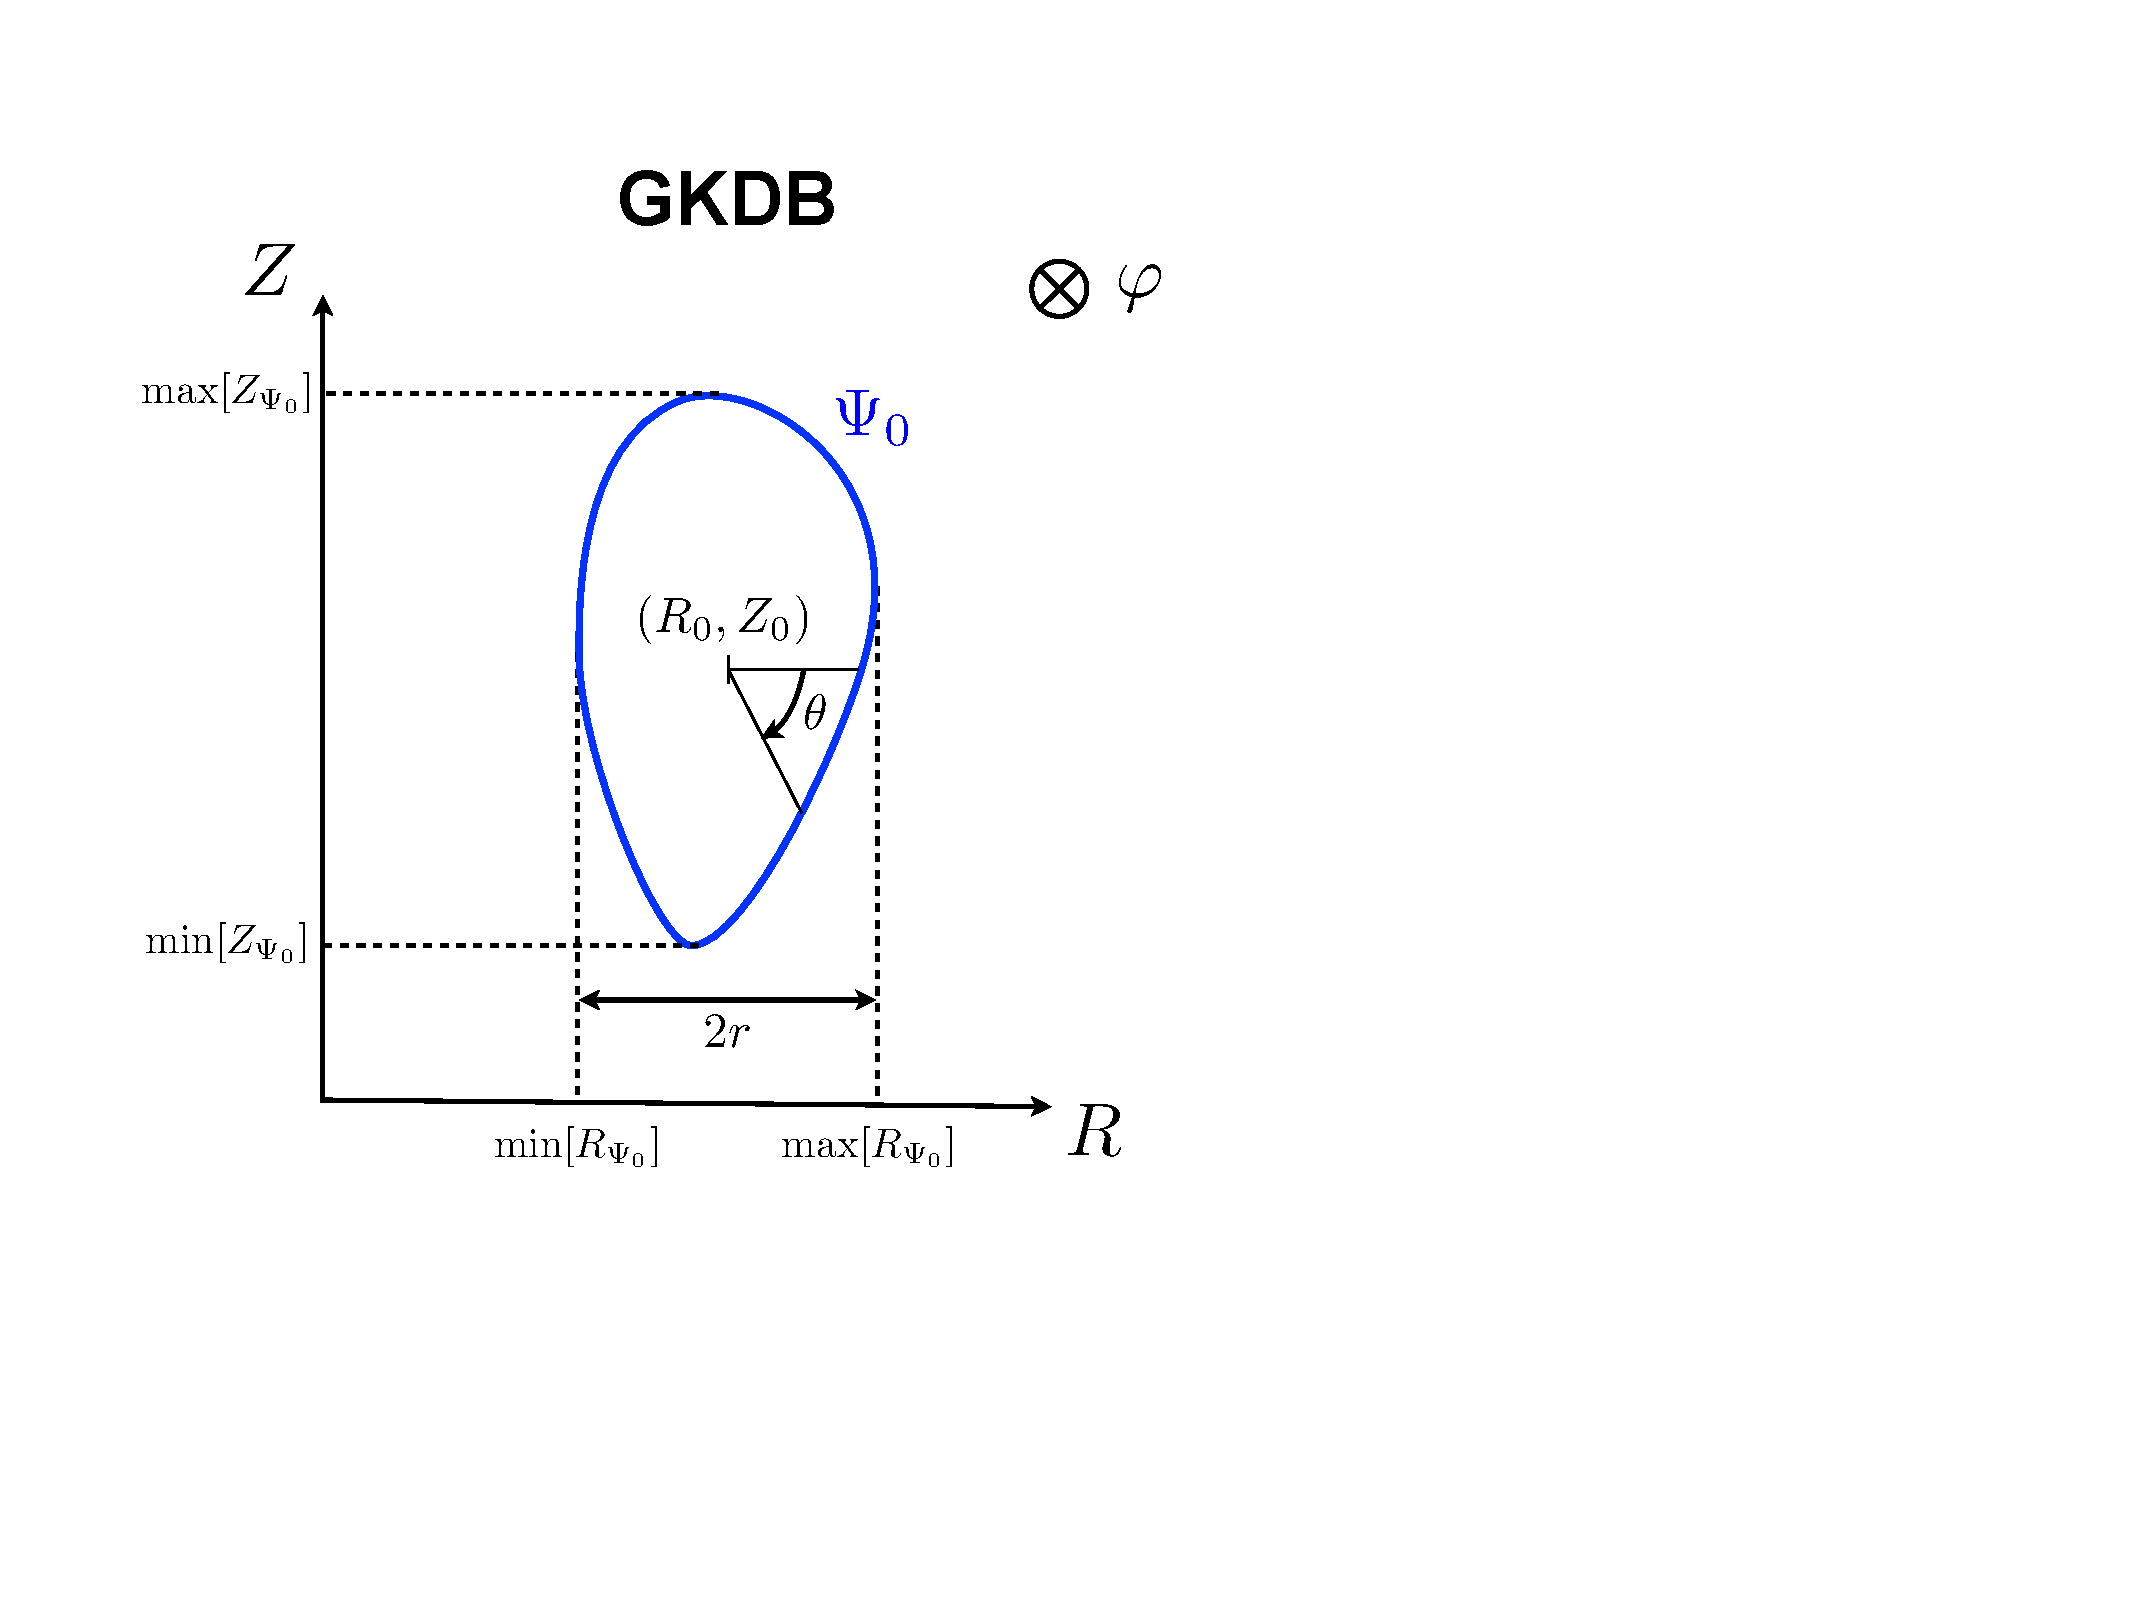
\includegraphics[width=7cm]{GKDB_coord.pdf}
		\caption{\label{fig:coord1} Cylindrical coordinate system used in GKW (left) and the GKDB (right).}
	\end{center}
\end{figure}\\
The flux surface centre definition depends on how the magnetic equilibrium is specified. For \texttt{miller} geometry, the definition of $R_0$ is identical to that used in the GKDB and $Z_0$ is given as an input in the geometry namelist:
\begin{equation}
R_0^\texttt{GKW-miller} = R_0^\gkdb \qquad \qquad Z_0^\texttt{GKW-miller} = \texttt{zmil}R_\tref^\gkw
\end{equation}
For \texttt{chease} geometry, $R_0$ is taken to be the value of \texttt{R0EXP} specified in the \texttt{hamada.dat} file and $Z_0$ is the elevation of the magnetic axis.
\begin{equation}
R_0^\texttt{GKW-chease} = \texttt{R0EXP} \qquad \qquad Z_0^\texttt{GKW-chease} = Z_\textrm{axis}
\end{equation}
The definition of the (dimensional) radial coordinate $r$ is identical in GKW and the GKDB:
\begin{equation}
r^\gkw = r^\gkdb
\end{equation}
The calculation of the  poloidal angle $\theta$ used in the GKDB from GKW inputs is documented in section~\ref{sec:magequil}. At this stage, just notice that most of the time $Z_0^\gkw\neq Z_0^\gkdb$, therefore, the points $s=0$ and $\theta=0$ do not necessarily coincide. 


\section{Reference quantities}
In GKW and the GKDB, all quantities are normalised and made dimensionless by making use of reference quantities. In what follows, normalised quantities are denoted with a "N" subscript. For instance, the normalised version of an arbitrary quantity $\mathcal{A}$ with the dimension of a length will be $\mathcal{A}_N^\gkw=\mathcal{A}/R_\tref^\gkw$ in GKW and $\mathcal{A}_N^\gkdb=\mathcal{A}/R_\tref^\gkdb$ in the GKDB. The conversion from GKW  to the GKDB  involves the ratio of reference quantities. For the example above:
\begin{equation}
\mathcal{A}_N^\gkdb = \frac{R_\tref^\gkw}{R_\tref^\gkdb} \mathcal{A}_N^\gkw
\end{equation}
The ratio of the various reference quantities used in GKW and the GKDB are:
\begin{align*}
q_\textrm{rat} &=  \frac{q_\tref^\gkw}{q_\tref^\gkdb} = - \frac{1}{\texttt{z}^\gkw_{e^-}} & R_\textrm{rat}^\texttt{miller} &= \frac{R_\tref^\texttt{GKW-miller}}{R_\tref^\gkdb} = 1 \\
m_\textrm{rat} &=  \frac{m_\tref^\gkw}{m_\tref^\gkdb} = \frac{m_e}{m_D}\frac{1}{\texttt{mass}^\gkw_{e^-}} & B_\textrm{rat}^\texttt{miller} &= \frac{B_\tref^\texttt{GKW-miller}}{B_\tref^\gkdb} = 1 \\
T_\textrm{rat} &=  \frac{T_\tref^\gkw}{T_\tref^\gkdb} = \frac{1}{\texttt{temp}^\gkw_{e^-}} &R_\textrm{rat}^\texttt{chease} &= \frac{R_\tref^\texttt{GKW-chease}}{R_\tref^\gkdb} = \frac{\texttt{R0EXP}}{R_0^\gkdb}  \\
n_\textrm{rat} &=  \frac{n_\tref^\gkw}{n_\tref^\gkdb} = \frac{1}{\texttt{dens}^\gkw_{e^-}} \frac{n_e(s=0)}{n_e(\theta=0)} & B_\textrm{rat}^\texttt{chease} &= \frac{B_\tref^\texttt{GKW-chease}}{B_\tref^\gkdb} = \frac{\texttt{B0EXP}}{B_0^\gkdb}
\end{align*}
where the $e^-$ subscript denotes the electron species and the electron to deuterium mass ratio is taken to be $\frac{m_e}{m_D}=2.7237 \times 10^{-4}$ in the GKDB.\\
The poloidal asymmetry factor for the density can be computed from data in the \texttt{cfdens} file (GKW output).  With \texttt{chease} geometry, the ratios $ L_\textrm{rat}$ and $ B_\textrm{rat}$ can be computed from data in the \texttt{hamada.dat} file (GKW input).


\chapter{Inputs}
\section{Magnetic equilibrium} \label{sec:magequil}
Only \texttt{miller} and \texttt{chease} magnetic equilibrium specifications are compatible with the GKDB format (\texttt{s-alpha} and \texttt{circ} are not an exact solution of the Grad-Shafranov equation).
\subsection{Flux surface centre}
Let's call $\{R_{\Psi_0},Z_{\Psi_0}\}$ a set of points discretizing the flux surface of interest. The values of $\{R_{\Psi_0},Z_{\Psi_0}\}/R_\tref^\gkw$ are available in the \texttt{geom.dat} file (GKW outpout) and can be used to compute $\{R_0^\gkdb,Z_0^\gkdb\}/R_\tref^\gkw$. 

\subsection{Poloidal angle}
With these values, one can then compute the GKDB poloidal angle $\theta$:
\begin{equation}
 \tan \theta = - \frac{Z_{\Psi_0}/R_\tref^\gkw-Z_0^\gkdb/R_\tref^\gkw}{R_{\Psi_0}/R_\tref^\gkw-R_0^\gkdb/R_\tref^\gkw}
\end{equation}
As the discretisation of the flux surface in \texttt{geom.dat} is done on the GKW $s$ grid, the equation above gives the relationship between $\theta$ and $s$.


\subsection{Plasma shape}



\chapter{Outputs}

\bibliographystyle{unsrt}
\bibliography{gkw2gkdb}

\end{document}
